\chapter{Dynamic plant--soil microbe interactions: the neglected effect of soil conditioning time: Appendices S1--S2}
%\chaptermark{Positive frequency-dependence}
%\renewcommand{\sectionmark}[1]{}
\fancyhead[LE, RO]{\thepage}
\fancyhead[RE]{APPENDIX E}
\fancyhead[LO]{TEMPORAL PLANT--SOIL FEEDBACK}
\fancyfoot{}
\renewcommand{\headrulewidth}{0pt}
\setlength{\parindent}{1cm}


\begin{comment}
\documentclass[hidelinks,letterpaper, 11pt]{article}
\usepackage{graphicx, bm, booktabs, lineno, array}
\usepackage[fleqn]{amsmath}
\usepackage{nicefrac}
\usepackage[compress,comma]{natbib}
\usepackage[right=1in, left=1in, top=1in, bottom=1in]{geometry}
\usepackage[parfill]{parskip}
\usepackage[usenames,dvipsnames]{color}
\usepackage[font=large,labelfont=bf,margin=1cm, labelsep = none]{caption} % caption formatting
\usepackage{setspace}
\usepackage{gensymb}
\usepackage{color}
\usepackage{sidecap}
%\usepackage{floatrow}
\usepackage{etoolbox}
\usepackage{tcolorbox}
\usepackage{newpxtext,newpxmath}
\tcbuselibrary{breakable}
%\usepackage{indentfirst}
\newbool{MyRefNumbers}
\usepackage{authblk}
\usepackage{hyperref}
\usepackage{mathpazo}
\usepackage[color=cyan, textsize=tiny]{todonotes}
\usepackage[font={normalsize}]{caption}
\usepackage{adjustbox}
\usepackage{array}
\usepackage{booktabs}
\usepackage{multirow}
\usepackage{tabularx}
% \usepackage{titling}

\setlength{\mathindent}{0pt}
\setlength{\parindent}{1cm}
% \makeatletter
% \makeatother
\pdfminorversion=3

% For table
\newenvironment{myindentpar}[1]%
{\begin{list}{}%
		{\setlength{\leftmargin}{#1}}%
		\item[]%
	}
	{\end{list}}
\newcommand*\samethanks[1][\value{footnote}]{\footnotemark[#1]}
\newcommand\blfootnote[1]{%
	\begingroup
	\renewcommand\thefootnote{}\footnote{#1}%
	\addtocounter{footnote}{-1}%
	\endgroup
}
\newcommand{\plus}{\raisebox{.4\height}{\scalebox{.6}{+}}}
\newcommand{\minus}{\raisebox{.4\height}{\scalebox{.8}{-}}}
% Command to recount supplement
\newcommand{\beginsupplement}{%
	\setcounter{table}{0}
	\renewcommand{\thetable}{S\arabic{table}}%
	\setcounter{figure}{0}
	\renewcommand{\thefigure}{S\arabic{figure}}%
}
% Command to center oversized images in floats
\newcommand{\centerfloat}{%
	\parindent \z@
	\leftskip \z@ \@plus 1fil \@minus \textwidth
	\rightskip\leftskip
	\parfillskip \z@skip}
\renewcommand\Affilfont{\fontsize{12}{12}\selectfont}
\newcommand{\ignore}[2]{\hspace{0in}#2}
\end{comment}



\begin{comment}
\begin{document}

\doublespacing
\title{Dynamic plant--soil microbe interactions: \\ the neglected effect of soil conditioning time}
\author[1, $\dagger$]{Po-Ju Ke}
\author[2]{Peter C. Zee}
\author[1, $\dagger$]{Tadashi Fukami}
\affil[1]{Department of Biology, Stanford University, Stanford, California, 94305, USA}
\affil[2]{Department of Biology, University of Mississippi, University, Mississippi, 38677, USA}
\date{\today}
\maketitle
\blfootnote{$\dagger$ Correspondence author: Department of Biology, Stanford University, Stanford, California 94305-5020, USA. Phone: +1 650-721-1711. Fax: +1 650-723-6132. Email: pojuke@stanford.edu, fukamit@stanford.edu}
	
\onehalfspacing
\noindent \textbf{Running title:} Temporal development of plant--soil feedback\\
\noindent \textbf{Keywords:} aerial photos, chronosequence, microbial community, plant--soil feedback, sand dunes, space-for-time substitution\\
\noindent \textbf{Type of article:} Letter\\
	
\begin{myindentpar}{1cm}
	\textbf{Words in Abstract:} 150\\
	\textbf{Words in main text:} $\sim$ 4000\\
	\textbf{Number of references:} 63\\
	\textbf{Number of figures:} 5\\
\end{myindentpar}
	
\noindent \textbf{Authorship statement:} PJK and TF conceived the study; PJK conducted the study and analyzed the data; PJK and PCZ developed the model and performed the simulation; PJK wrote the first draft of the manuscript with substantial contribution from all authors.\\
	
\noindent \textbf{Data accessibility statement:} Should the manuscript be accepted, all data and computer scripts supporting the results will be archived in a public Github repository, with the DOI included at the end of the article.\\

\linenumbers
\doublespacing
\end{comment}



\section{Appendix S1 -- Detailed methods}
\subsection{DNA sequencing of fungal and bacterial communities}
We extracted microbial DNA from 0.25 g of subsampled soil with PowerSoil DNA Isolation Kit (Qiagen) following the manufacturer's protocol. We then amplified the bacterial 16S ribosomal DNA region, with primer pair 515f (5$^\prime$- GTG YCA GCM GCC GCG GTA A -3$^\prime$) -- 806r (5$^\prime$- GGA CTA CNV GGG TWT CTA AT -3$^\prime$) \citep{Caporaso2012}, and the fungal internal transcribed spacer 1 region (ITS1), with primer pair ITS1-F$\textunderscore$KYO1 (5$^\prime$- CTH GGT CAT TTA GAG GAA STA A -3$^\prime$) -- ITS2$\textunderscore$KYO2 (5$^\prime$- TTY RCT RCG TTC TTC ATC -3$^\prime$) \citep{Toju2012}. Each primer was concatenated with 3 -- 6-mer Ns \citep{Lundberg2013} and an Illumina sequencing primer region, resulting in a fusion primer for our PCR reactions (forward: 5$^\prime$- TCG TCG GCA GCG TCA GAT GTG TAT AAG AGA CAG -- [3--6-mer Ns] -- [515f or ITS1-F$\textunderscore$KYO1] -3$^\prime$; reverse: 5$^\prime$- GTC TCG TGG GCT CGG AGA TGT GTA TAA GAG ACA G -- [3--6-mer Ns] -- [806r or ITS2$\textunderscore$KYO2] -3$^\prime$). 
\par


Our 10 $\mu$L PCR reaction contained 3.2 $\mu$L of MQ water, 5 $\mu$L of MyTaq HS DNA polymerase Mastermix (Bioline), 0.4 $\mu$L of each primer (10$\mu$M for both forward and reverse primer), and 1 $\mu$L of extracted DNA. We ran the reactions at 95$^{\circ}$C for 2 min, followed by 36 cycles of 95$^{\circ}$C for 20 sec, 52.5$^{\circ}$C for 16S (or 50$^{\circ}$C for ITS1) for 20 sec, 72$^{\circ}$C for 50 sec, and a final extension at 72$^{\circ}$C for 10 min. A ramp rate of 1$^{\circ}$C/s was set to prevent chimeric amplicon generation. After this first PCR process, we ran a subsequent second PCR for sample identification. The fusion primers used in this second PCR concatenates P5/P7 Illumina adaptors, 8-mer index sequences, and the sequencing adaptor \citep{Hamady2008} (forward: 5$^\prime$- AAT GAT ACG GCG ACC ACC GAG ATC TAC AC -- [8-mer tag] -- TCG TCG GCA GCG TC -3$^\prime$; reverse: 5$^\prime$- CAA GCA GAA GAC GGC ATA CGA GAT -- [8-mer tag] -- GTC TCG TGG GCT CGG -3$^\prime$). The second PCR was run for 8 cycles with the same temperature profile as our first PCR but with an annealing temperature of 50$^{\circ}$C for both bacterial 16S and fungal ITS1 amplicons. After a purification/equalization process with the AMPure XP Kit (with a sample : AMpureXP ratio = 1 : 0.6, Agencourt), 5$\mu$L of PCR product were taken from each sample to create a pooled library. This library was then sequenced using the Illumina MiSeq sequencer at the Stanford Functional Genomics Facility (2 $\times$ 250 cycle sequencing kit) with 15$\%$ PhiX spike-in.
\par


The raw Illumina MiSeq sequencing reads were processed with the Claident pipeline (\citealp{Tanabe2013}, v0.2.2015.11.19). To prevent potential mis-tagging, demultiplexing was conducted within Claident after converting raw Miseq BCL data into FASTQ data with the program bcl2fastq v1.8.4. All sequencing reads with low quality scores ($<$ 30) were deleted. The obtained forward and reverse sequencing reads were fused with each other by the program PEAR v0.9.6 \citep{Zhang2014} and merged reads with low quality (quality score $<$ 30 or length $<$ 150 bp) were deleted. Potentially chimeric and noisy reads were also eliminated with the program UCHIME v4.2 \citep{Edgar2011}. Sequencing reads that passed through all filtering processes were then clustered into operational taxonomic units (OTUs), with a cutoff sequence similarity of 97$\%$, with the program VSEARCH (\citealp{Rognes2016}, implemented in Claident). This clustering process resulted in 19,868 OTUs representing 1,772,220 sequences for ITS1 sequencing reads and 164,983 OTUs representing 3,512,717 sequences for 16S sequencing reads. After clustering, fungal and bacterial OTUs with less than ten total sequencing reads were removed. Taxonomy was assigned to the remaining OTUs using the RDP Naive Bayesian rRNA Classifier v2.11 \citep{Wang2007} trained on either the 16S rRNA training set 16 for bacteria or the Warcup Fungal ITS training set 2 \citep{Deshpande2016} for fungi. Based on the taxonomic assignment results, ITS1(16S) sequences other than those of the Kingdom fungi (bacteria) were removed from the dataset. For both ITS and 16S datasets, potential contaminant OTUs were identified statistically based on their prevalence in PCR and extraction negative controls (two of each for every 96 well plate reaction) using the R package decontam \citep{Davis2018}.This resulted in the elimination of 36 fungal ITS and 22 bacterial 16S OTUs. Finally, before any downstream analyses presented in this study, the OTU tables were rarefied to 1,000 sequencing reads \citep{McMurdie2013}. For fungal communities, the rarefaction process deleted 1 \textit{B. pilularis} individual and 6 sand samples.
\par


\subsection{Statistical analysis of microbial communities}
To identify the fungal and bacterial taxonomic groups that are driving the observed community pattern, we applied a model-based approach with the R package HMSC \citep{Ovaskainen2017}. 
To ensure adequate model fit, we aggregated the microbial communities to the family level and constrained this analysis to fungal and bacterial families that belonged to the top ten abundant phyla and occurred in more than 20$\%$ of the samples. 
Different from other analyses, this model fitting was performed by treating each soil sample as replicate units in order to take advantage of the hierarchical Bayesian approach implemented in \textit{HMSC} \citep{Ovaskainen2017}. 
We assumed that the abundance of each fungal and bacterial class follows an over-dispersed Poisson distribution and fitted models with plant age as fixed effect and plant individual as random effect. 
For all models, the MCMC sampling was conducted for 1,000,000 iterations, with a burn-in phase of 500,000 iterations and thinned every 100 iterations.
All model fitting was performed separately for each plant species. This is because plants vary in their longevity and thus the same age does not necessarily represent the same life stage for different plants.
The mean and the 95$\%$ credible interval of the age coefficient's marginal posterior distributions were summarized and plotted for each plant species separately.
\par


\subsection{Greenhouse experiment}
Our greenhouse experiment used soil samples collected in July 2017 and was separated into two rounds, which started in late August and September 2017, respectively. The range and variance of age of individuals were kept similar among the two rounds. To avoid arbitrarily averaging soil conditions \citep{Rinella2018}, soils collected from different individuals were kept separated throughout the experiment. Half of the volume (150 mL) collected from each individual was autoclaved to create a sterile treatment (120$^\circ$C for 60 min, sit overnight for 24 h, and another 120$^\circ$C for 60 min). Due to handling mistakes, we had to discard soil inocula collected from 9 individuals: 6 in the first round (i.e., soils from 1 individual of \textit{A. arenaria}, 3 individuals of \textit{C. edulis}, and 2 individuals of \textit{L. arboreus}), and 3 in the second round (i.e., soils from 2 individuals of \textit{B. pilularis} and 1 individual of \textit{C. edulis}). Two rounds combined, we ended up with 222 unique soil environments: 108 in the first round (i.e., (14 \textit{A. arenaria} + 15 \textit{B. pilularis} + 12 \textit{C. edulis} + 13 \textit{L. arboreus}) individuals $\times$ 2 sterilization treatments), and 114 in the second round (i.e., (15 \textit{A. arenaria} + 13 \textit{B. pilularis} + 14 \textit{C. edulis} + 15 \textit{L. arboreus}) individuals $\times$ 2 sterilization treatments).
\par


Plant seeds were purchased from commercial seed suppliers (i.e., \textit{A. arenaria}: Jelitto perennial seeds; \textit{B. pilularis}: Larner seeds; \textit{C. edulis}: independent donor; \textit{L. arboreus}: J.L. Hudson, Seedsman). The seeds were surface sterilized by soaking seeds in 5$\%$ bleach for 30 sec, 95$\%$ ethanol for 30 sec, and rinsing them with DI water for 1 min. The sterilized seeds were spread evenly onto germination trays filled with sterilized sand (1:1 mixing of sterile play sand and Lapis Lustre $\#$ 2/12 sand (Cemex) to mimic the soil particle distribution in the field), and placed in a growth chamber (16-hr/8-hr light/dark, and temperature held at 16$^\circ$C). After two weeks, we transplanted the seedlings individually into 107 mL "cone-tainers" pots (hereafter "pots"; Stuewe and Sons) filled with 80 mL of sterilized sand (prepared with the same method as for germination) and added 20 mL of either live or sterile soil inoculum to the top. Three of the four species were transplanted in both experimental rounds, with \textit{B. pilularis} being the exception due to low germination rate during the second round. The final number of pots was 774, consisting of 432 from the first round (i.e., 54 individuals $\times$ 2 sterilization treatments $\times$ 4 species) and 342 from the second round (i.e., 57 individuals $\times$ 2 sterilization treatments $\times$ 3 species).
\par

 
Transplanted pots were randomly placed onto every other cell of 98 well trays (to avoid crowding), and were grown in the greenhouse for 12 weeks (14-hr/10-hr light/dark with ambient temperature). To mimic precipitation regimes in the field, which is mainly fog during the summers, 30 sec brief water spray with automatic misting nozzles were applied every hour. Seedlings that died within the first 10 days were replanted, and for seedlings that died afterwards their live--sterile soil pair were discarded from the calculation of microbial effects. Two rounds combined, data for 20 live--sterile soil pairs were discarded due to the death of seedlings or handling mistakes: 3 seedlings of \textit{A. arenaria} (i.e., 1 in \textit{A. arenaria} soil, 1 in \textit{B. pilularis} soil, 1 in \textit{L. arboreus} soil), 5 seedlings of \textit{B. pilularis} (i.e., 2 in \textit{A. arenaria} soil, 1 in \textit{B. pilularis} soil, 1 in \textit{C. edulis} soil, 1 in \textit{L. arboreus} soil), 9 seedlings of \textit{C. edulis} (i.e., 2 in \textit{A. arenaria} soil, 3 in \textit{B. pilularis} soil, 2 in \textit{C. edulis} soil, 2 in \textit{L. arboreus} soil), and 3 seedlings of \textit{L. arboreus} (i.e., 1 in \textit{B. pilularis} soil, 1 in \textit{C. edulis} soil, 1 in \textit{L. arboreus} soil). After 12 weeks, we harvested all above- and below-ground tissue from each pot, carefully rinsed soil off the root system, and oven-dried tissue at 70$^{\circ}$C for 96 h. 
% Ambient temperature for August--September: mean daily maximum is 29.8$^\circ$C and mean daily  minimum is 18.1$^\circ$C,
\par



\subsection{Simulation model}
\subsubsection*{Overview}
To investigate the potential long-term effects of temporally-varying plant--soil microbe interactions on plant community dynamics, we constructed an individual-based model following the model in  \citet{FukamiNakajima2011} (see also \citealp{Fukami2013, ZeeFukami2015, Fukami2017}). The model simulates the immigration, reproduction, arrival, establishment, and death of plant individuals. 
In our model, plant propagules consist of immigration from a regional species pool and seed production dispersed from established plants. These propagules compete for the establishment at empty sites, where species' competitive ability is determined by the habitat condition of the site, species' trait, and the legacy soil microbial effects (i.e., plant--soil microbe interactions) imposed by the previously established plant species. 
Established individuals die with a fixed mortality rate and those that survived can produce propagules next year to colonize empty sites, which are released as individuals die.
We simulated the community assembly process for multiple years, repeating the above processes until a stable state was reached. All simulation runs were performed in \textit{R} version 3.3.1 \citep{R}. 
\par


\subsubsection*{Species pool and landscape}
For each round of simulated community assembly, we considered a regional species pools containing 50 plant species. Each species $i$ is characterized by a trait value, $R_{i}$, chosen randomly from a uniform distribution $U\left ( 0, 1 \right )$. Species are also characterized by a set of plant--soil microbe interaction values, $S_{ij}^{\tau}$. These values quantify how the previously-established plant species $j$, which died at age $\tau$, affect the competitive ability of plant species $i$ (see section \textit{Plant-soil interactions}). 
One patch in our simulation consists of 1024 local sites, arranged in a one-dimensional circular array, for plant individuals to colonize. Local site are characterized by a habitat condition value, $H_{k}$, chosen randomly from a beta-distribution with shape parameters $\alpha = \beta = 50$. This setting yielded many local sites having $H_{k}$ values close to 0.5 and few close to either 0 or 1. 
\par


\subsubsection*{Community assembly}
We started our simulation from an empty patch, allowing plant propagules to colonize empty local sites. In our model, plant propagules consist of immigrants from the regional species pool and seeds produced and dispersed from established plants.
Each year, species in the regional species pool immigrate to the patch with equal probability, $p_{I} = 0.05$. Selected immigrating species produce $f_{I} = 10$ propagules that disperse globally, i.e., the propagule can land at any local site with equal probability.
In addition to immigration, established individuals contribute to the propagule rain by seed production. We assumed that all established individuals reproduce at each time step (i.e., $p_{R} = 1$) and reproducing individuals have a fecundity of $f_{R} = 5$.
We assumed that seeds produced by established individuals have limited dispersal ability: the landing locations of seeds were drawn independently from a Gaussian distribution with a mean at the location of its reproducing parent and a variance of $\sigma_{R}$, which determines how far seeds can disperse. We set $\sigma_{R} = 150$ to represent intermediate dispersal distance \citep{ZeeFukami2015}.
Propagules that landed at local sites with an established individual will perish as they cannot displace the resident, whereas those that landed at an empty local site would have a chance to establish.
To highlight the effects of soil microbial legacies, demographic parameters mentioned above were set equal for all species.
\par


When more than one propagule landed at the same empty site, the propagule belonging to the species with the highest value of competitiveness, $C_{ijk}^{\tau}$, will successfully establish. 
Modified from \citet{Fukami2013}, we defined $C_{ijk}^{\tau}$ of species $i$ at site $k$, which was made vacant during the previous time step when species $j$ died, as $C_{ijk}^{\tau} = \left ( 1 - \left | H_{k} - Z_{i} \right | \right )S_{ij}^{\tau}$. 
The term within the parenthesis measures the relative fit of species $i$ to the habitat condition at site $k$, i.e., species with a closer trait value--habitat condition match are superior competitors. 
This term is modulated by $S_{ij}^{\tau}$, which captures the soil microbial legacy effect that an aged-$\tau$ species $j$ individual imposes on the newly-arrived species $i$ propagule. The superscript $\tau$ indicates the age-at-death, and thus the length of soil conditioning, of species $j$, which is an important determinant of the plant--soil microbe interaction strength (see section \textit{Plant-soil interactions}).
After competition for establishment was completed, individuals die with a mortality rate, $m$, which is set equal as 0.2 for all species. As we assumed replacement competition, an established individual will persist until its stochastic death, regardless of whether more competitive propagules arrive later at its site.
We assembled communities by following these rules of immigration, reproduction, arrival, establishment, and death for $t = 2000$ years. 
\par


\subsubsection*{Age-dependent plant--soil interactions}
The value of $S_{ij}^{\tau}$ captures the direction and strength of soil microbial legacy effects that an individual of species $j$, which died at the age of $\tau$, imposes on species $i$. A value of 1 indicates no microbial effects as it does not modify the competitiveness of species $i$. A value greater than 1 indicates positive microbial effects (e.g., facilitation through beneficial microbes), whereas a value less than 1 indicates negative microbial effects (e.g., antagonism through detrimental pathogens). Following \citet{Fukami2013}, we considered four types of plant--soil microbe interactions: 
(1) `no interactions', where $S_{ij}^{1}$ (i.e., the baseline microbial effect generated by an individual that only survived for one year) is 1 for all pairs of species $i$ and $j$; 
(2) `positive conspecific interactions', where $S_{ij}^{1}$ is chosen randomly from a uniform distribution $U\left ( 1.0, 1.5 \right )$ when $i = j$ but equals 1 when $i \neq j$; 
(3) `negative conspecific interactions', where $S_{ij}^{1}$ is chosen randomly from $U\left ( 0.5, 1.0 \right )$ when $i = j$ but equals 1 when $i \neq j$; 
(4) `complex plant--soil microbe interactions', where $S_{ij}^{1}$ is chosen randomly from $U\left ( 0.5, 1.0 \right )$ when $i = j$ and from $U\left ( 0.5, 1.5 \right )$ when $i \neq j$ (i.e., conspecific interactions are negative whereas heterospecific ones can be either positive or negative).
\par


To incorporate age-dependent plant--soil microbe interactions, we considered four temporal development scenarios of $S_{ij}^{\tau}$: 
(1) `constant', where the microbial effect remains at its baseline $S_{ij}^{1}$ value and is independent to the age-at-death, $\tau$, of the individual of species $j$; 
(2) `magnifying', where positive and negative microbial effects intensify in their strengths with greater age-at-death of the individual of species $j$ (i.e., $S_{ij}^{\tau}$ start from its baseline $S_{ij}^{1}$ value and intensify towards its biological extremes, 1.5 and 0.5 for positive and negative microbial effects, respectively, with increasing $\tau$); 
(3) `decaying', where positive and negative microbial effects attenuate with greater age-at-death of the individual of species $j$ (i.e., $S_{ij}^{\tau}$ start from its baseline $S_{ij}^{1}$ value and decay towards 1 with increasing $\tau$); 
(4) `bidirectionally varying', where $S_{ij}^{1}$ has equal probability to either intensify (towards biological extremes) or attenuate (towards no feedback) with increasing $\tau$.
For scenarios (2)--(4), we assumed that changes in $S_{ij}^{\tau}$ follow a linear function and set the rate of change to 0.1 per year. 
A schematic description of microbial effects varying through time is given in Fig.~\ref{fig:SimulationComplexPSF}.
\par


\subsubsection*{Simulation exercise and calculating species diversity}
We focused on the effects of different temporal development scenarios on plant community convergence.
For each of the four plant--soil microbe interactions types (i.e., no interactions, positive, negative, and complex interactions), we generated one set of baseline plant--soil interaction matrix (i.e., $S_{ij}^{1}$ values) and ran simulations with $S_{ij}^{\tau}$ values following different temporal development scenarios (i.e., constant, magnifying, decaying, and bidirectionally varying).
In total, our simulation resulted in 13 interaction type $\times$ temporal development combinations since the no interaction simulations can only remain constant through time.
For our whole simulation exercise, we generated 10 patches for the regional species pools to colonize independently and quantified changes in species diversity indexes through time. 
We measured alpha-diversity as the average number of species presented in the 10 patches, and gamma-diversity as the number of species presented in at least one patch. We measured beta-diversity as the gamma-diversity divided by the averaged alpha-diversity, which can be viewed as a proxy of the effective number of distinct local communities in the region \citep{FukamiNakajima2011}.
For each interaction type $\times$ temporal development combination, the above simulation was replicated 20 times, where 20 independently-created sets of regional species pool were allowed to colonize the same set of 10 patches, using the same set of $S_{ij}^{1}$ values for each plant--soil microbe interaction type. We then compared the mean beta-diversity and the temporal trajectory among different temporal development scenarios.
\par



\clearpage
\section{Appendix S2 -- Supplementary Figures}
\begin{figure}[h]
	\centering
	\makebox[\textwidth][c]{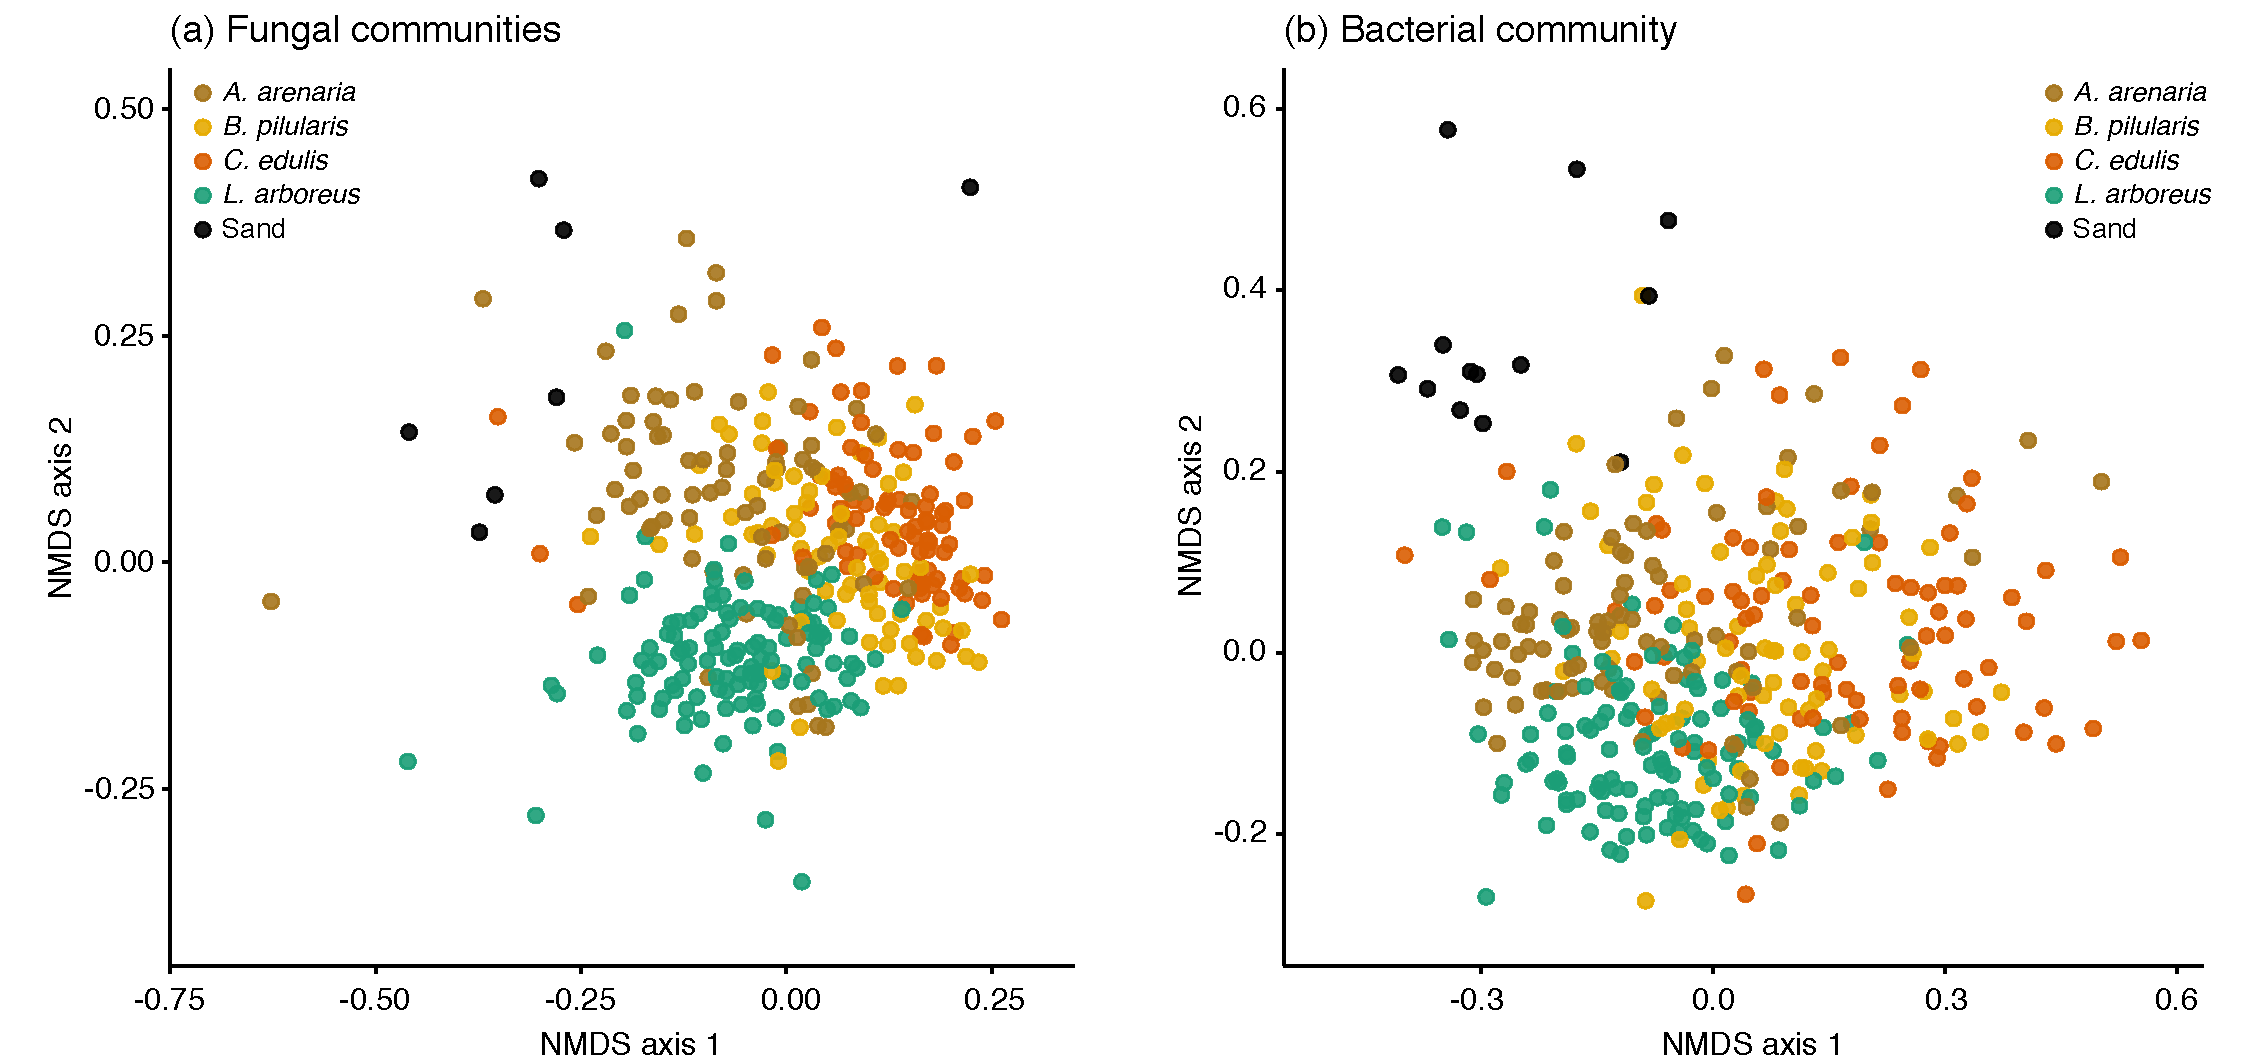
\includegraphics[width=15cm]{Chapter6/Composition_Both_Species.pdf}}
	\caption[NMDS ordination of all (a) fungal and (b) bacterial communities.]
		{\hspace{1mm} 
		NMDS ordination of all (a) fungal and (b) bacterial communities. Points are color-coded based on the identity of the plant species: \textit{A. arenaria} (brown); \textit{B. pilularis} (yellow); \textit{C. edulis} (orange); \textit{L. arboreus} (green); sand (black). 
		Statistics were performed at the plant individual level, but for visualization purpose each point represents the bacterial community of one soil sample. Panel (a) and (b) are the same ordination plot as in Figs \ref{fig:FunComposition} and \ref{fig:BacComposition}, respectively.}
	\label{fig:BothComposition}
\end{figure}



\newpage
\begin{figure}[h]
	\centering
	\makebox[\textwidth][c]{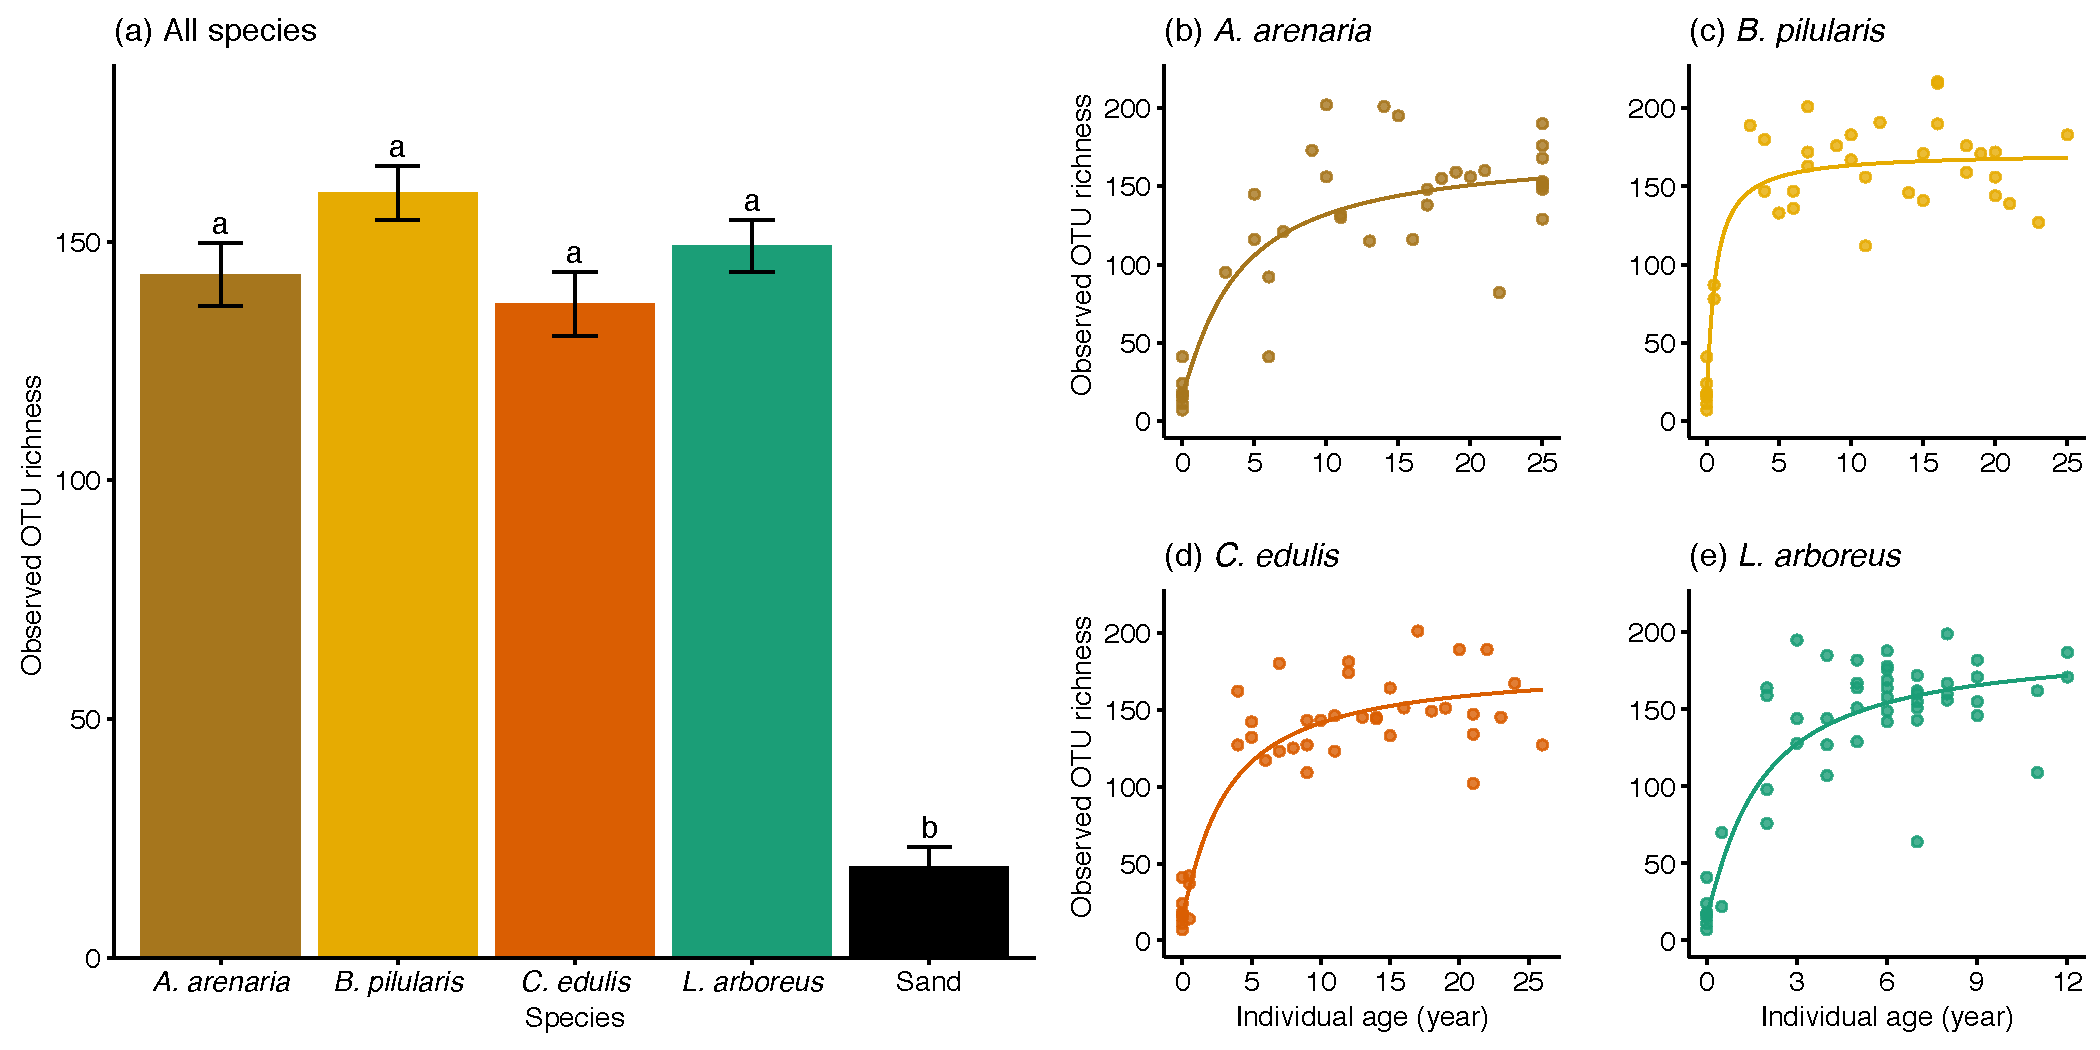
\includegraphics[width=15cm]{Chapter6/Richness_Fungi_Summary.pdf}}
	\caption[Fungal community richness as a function of plant age.]
		{\hspace{1mm} 
		Fungal community richness as a function of plant age. (a) Species-specific difference in observed fungal OTU richness. 
		(b)-(e) Temporal trend of observed richness with increasing plant age for each plant separately. (b) \textit{A. arenaria} (brown); (c) \textit{B. pilularis} (yellow); (d) \textit{C. edulis} (orange); (e) \textit{L. arboreus} (green). 
		Different letters in (a) represent significant difference among plant species. Each point in panels (b)-(e) represents the aggregated fungal community from one plant individual. A Monod function was the best fit for the temporal pattern: $\text{richness} = \mu \times \tfrac{\text{age}}{K + \text{age}} + m$, where $\mu$ is the maximum rate of richness increase, $K$ is the half-saturation constant, and $m$ is the minimum level offset.}
	\label{fig:FunRichness}
\end{figure}



\newpage
\begin{figure}[h]
	\centering
	\makebox[\textwidth][c]{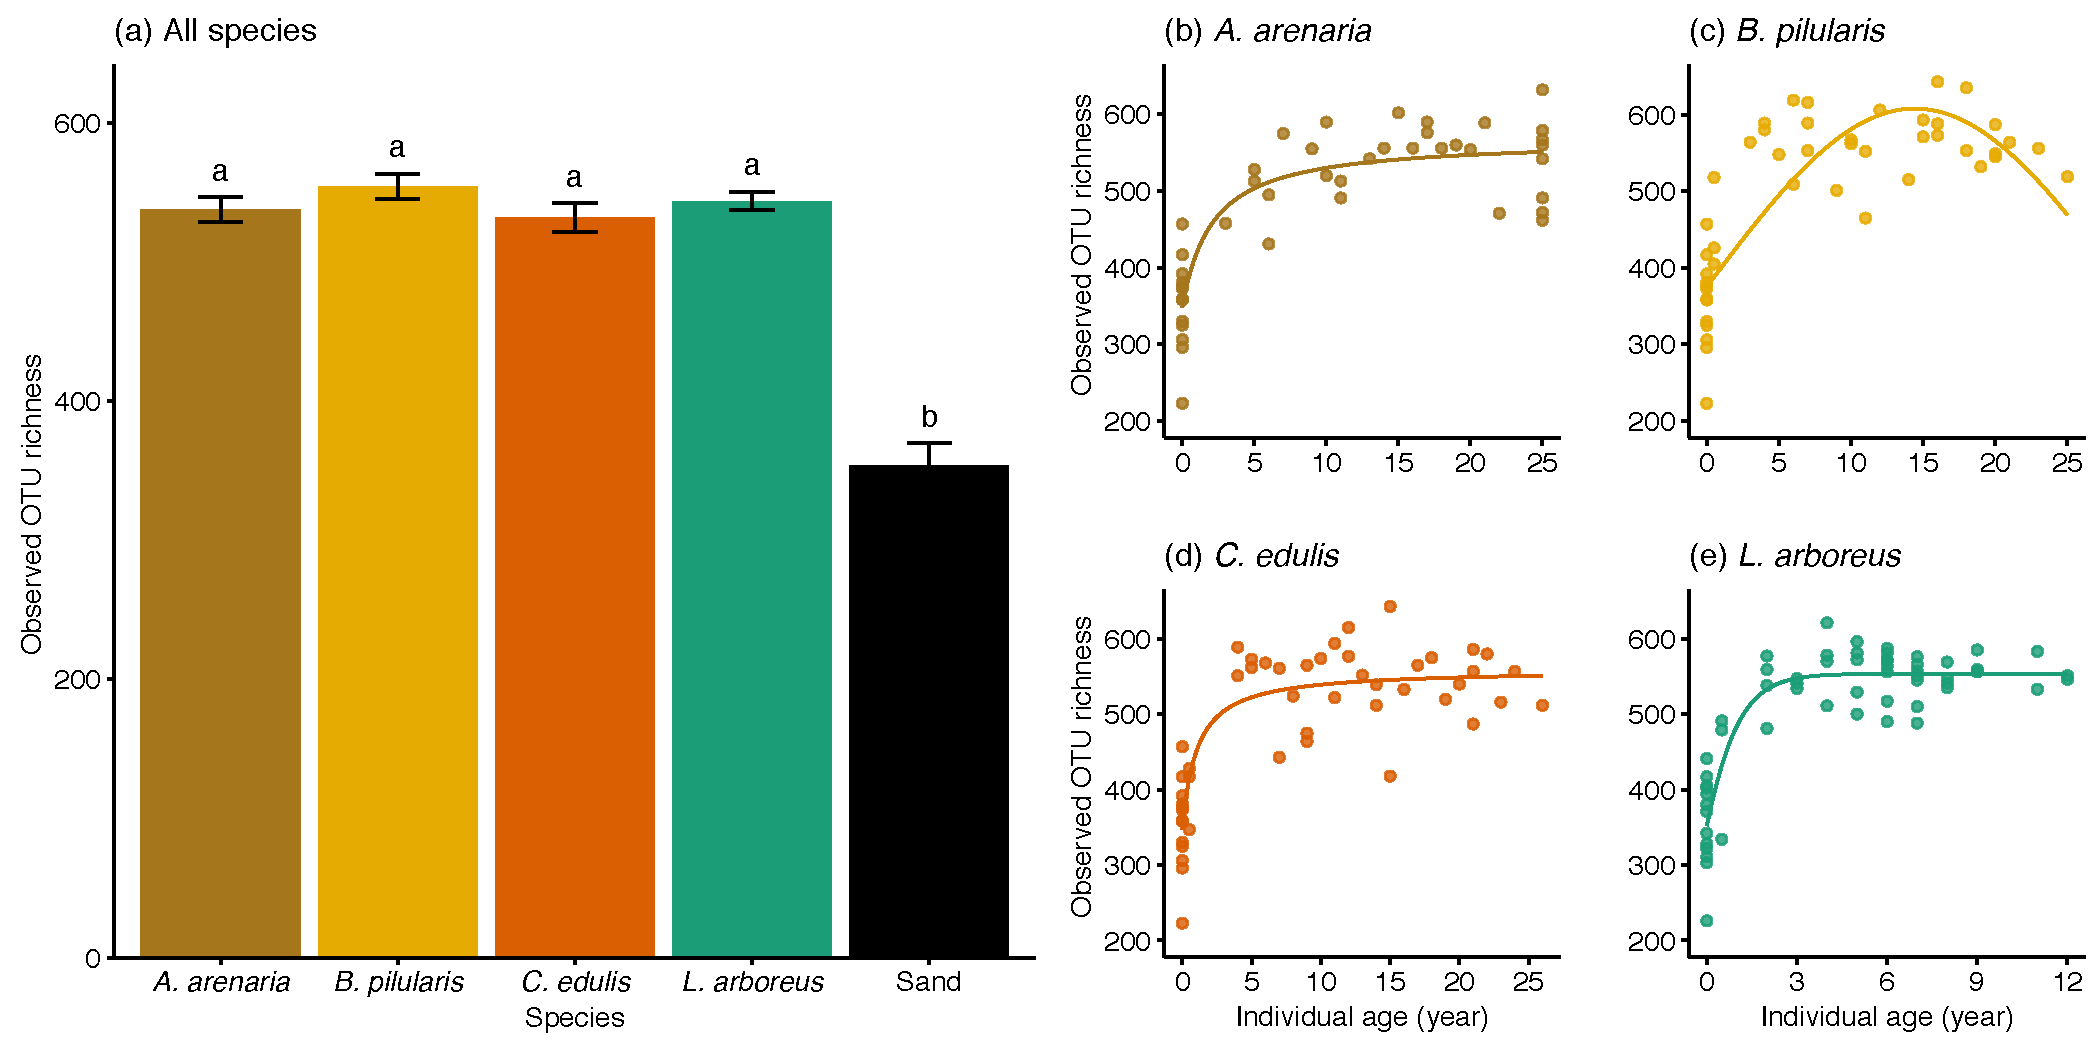
\includegraphics[width=15cm]{Chapter6/Richness_Bacteria_Summary.pdf}}
	\caption[Bacterial community richness as a function of plant age.]
		{\hspace{1mm} 
		Bacterial community richness as a function of plant age. (a) Species-specific difference in observed bacterial OTU richness.
		(b)-(e) Temporal trend of observed richness with increasing plant age for each plant separately. (b) \textit{A. arenaria} (brown); (c) \textit{B. pilularis} (yellow); (d) \textit{C. edulis} (orange); (e) \textit{L. arboreus} (green). 
		Different letters in (a) represent significant difference among plant species. Each point in panels (b)-(e) represents the aggregated bacterial  community from one plant individual. A quadratic function was the best fit for \textit{B. pilularis}, whereas a Monod function was the best fit for the other three species.}
	\label{fig:BacRichness}
\end{figure}



\newpage
\begin{figure}[h]
	\centering
	\makebox[\textwidth][c]{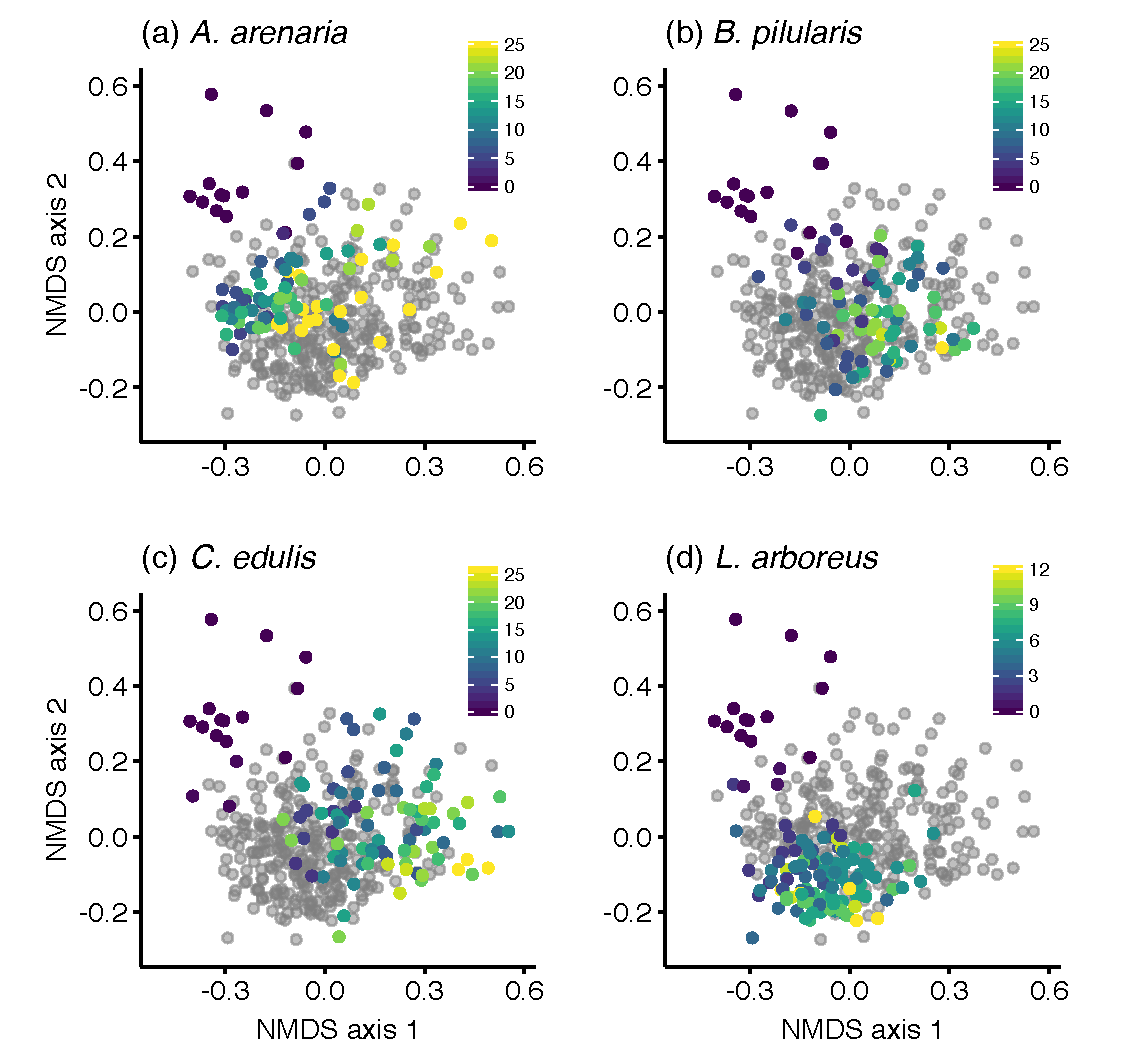
\includegraphics[width=14cm]{Chapter6/Composition_Bacteria_Age.pdf}}
	\caption[Bacterial community composition as a function of plant species and the age of plant individuals.]
		{\hspace{1mm} 
		Bacterial community composition as a function of plant species and the age of plant individuals. Each panel highlights one focal plant species on the NMDS ordination plot of all bacterial communities. Bacterial communities associated with the focal species are color-coded by individual plant age, whereas the other three species are in gray. Purple to yellow represent the age gradient from young to old, with species-specific minimum and maximum age. (a) \textit{A. arenaria}; (b) \textit{B. pilularis}; (c) \textit{C. edulis}; (d) \textit{L. arboreus}. 
		Statistics were performed at the plant individual level, but for visualization purpose each point represents the bacterial community of one soil sample. Note that dark purple points that appeared in all panels represent bacterial communities associated with bare sand. See the same ordination plot but color-coded with species identity in Fig.~\ref{fig:BothComposition}b.}
	\label{fig:BacComposition}
\end{figure}



\newpage
\begin{sidewaysfigure}[h]
	\centering
	\makebox[\textwidth][c]{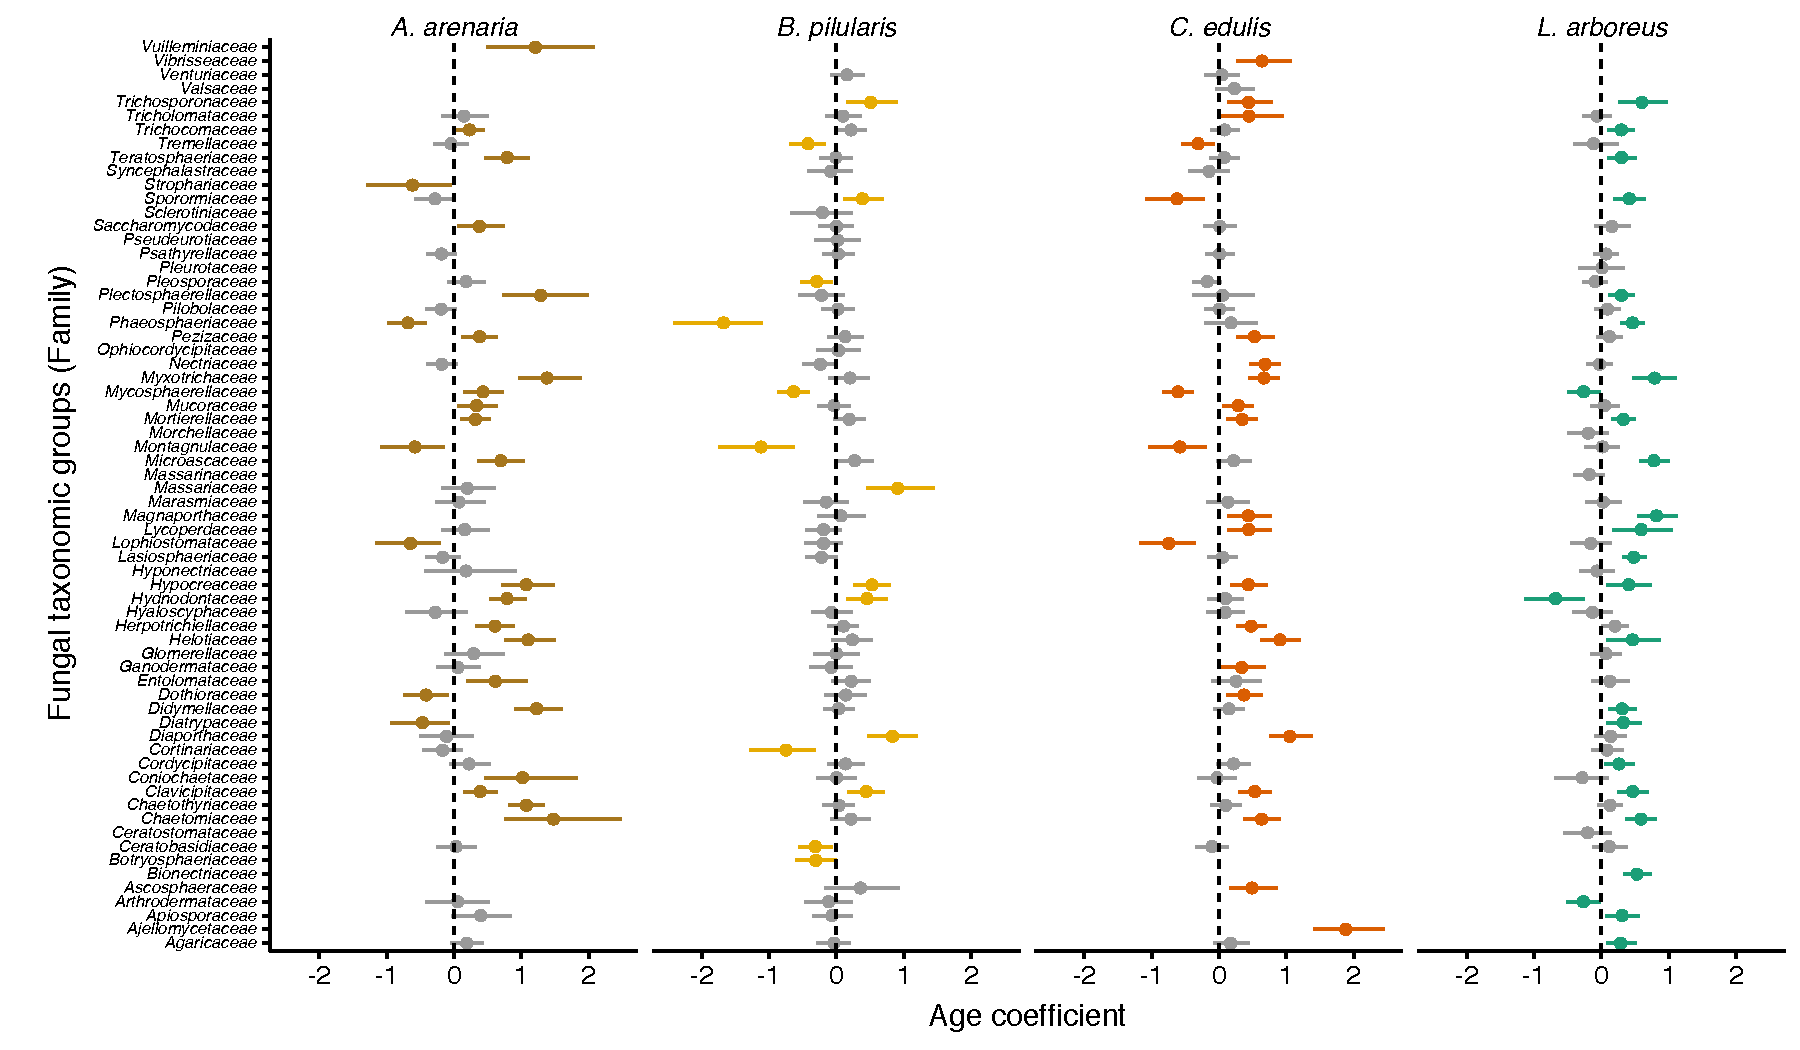
\includegraphics[width=20cm]{Chapter6/HMSC_Fungi_Family_Summary.pdf}}
	\caption[HMSC results demonstrating which fungal families show significant temporal trends.]
		{\hspace{1mm} HMSC results demonstrating which fungal families show significant temporal trends. Points and line segments represent the mean and the 95$\%$ credible interval of the fitted age coefficient for different fungal families (y-axis). All model fitting were performed separately for each plant species, from left to right: \textit{A. arenaria} (brown); \textit{B. pilularis} (yellow); \textit{C. edulis} (orange); \textit{L. arboreus} (green).}
	\label{fig:FunHMSC}
\end{sidewaysfigure}



\newpage
\begin{sidewaysfigure}[h]
	\centering
	\makebox[\textwidth][c]{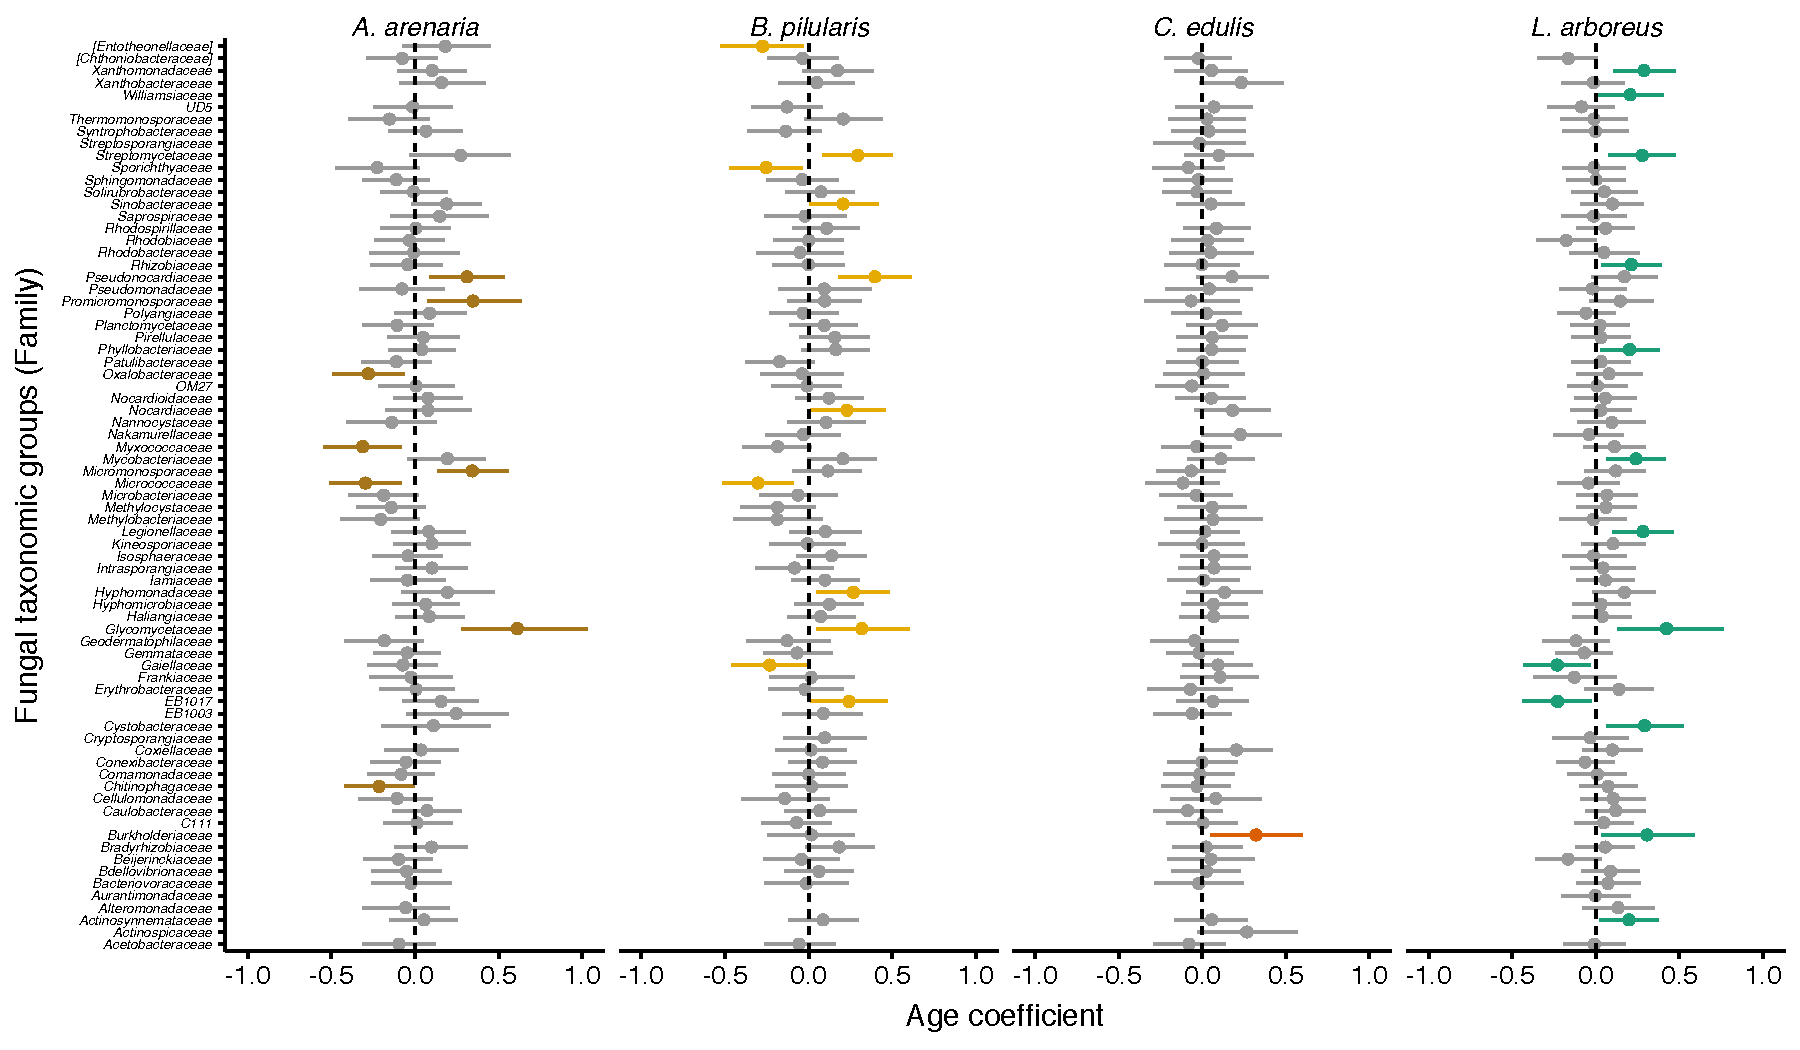
\includegraphics[width=20cm]{Chapter6/HMSC_Bacteria_Family_Summary.pdf}}
	\caption[HMSC results demonstrating which bacterial families show significant temporal trends.]
		{\hspace{1mm} HMSC results demonstrating which bacterial families show significant temporal trends. Points and line segments represent the mean and the 95$\%$ credible interval of the fitted age coefficient for different bacterial families (y-axis). All model fitting were performed separately for each plant species, from left to right: \textit{A. arenaria} (brown); \textit{B. pilularis} (yellow); \textit{C. edulis} (orange); \textit{L. arboreus} (green).}
	\label{fig:BacHMSC}
\end{sidewaysfigure}



\newpage
\begin{sidewaysfigure}[h]
	\centering
	\makebox[18cm][c]{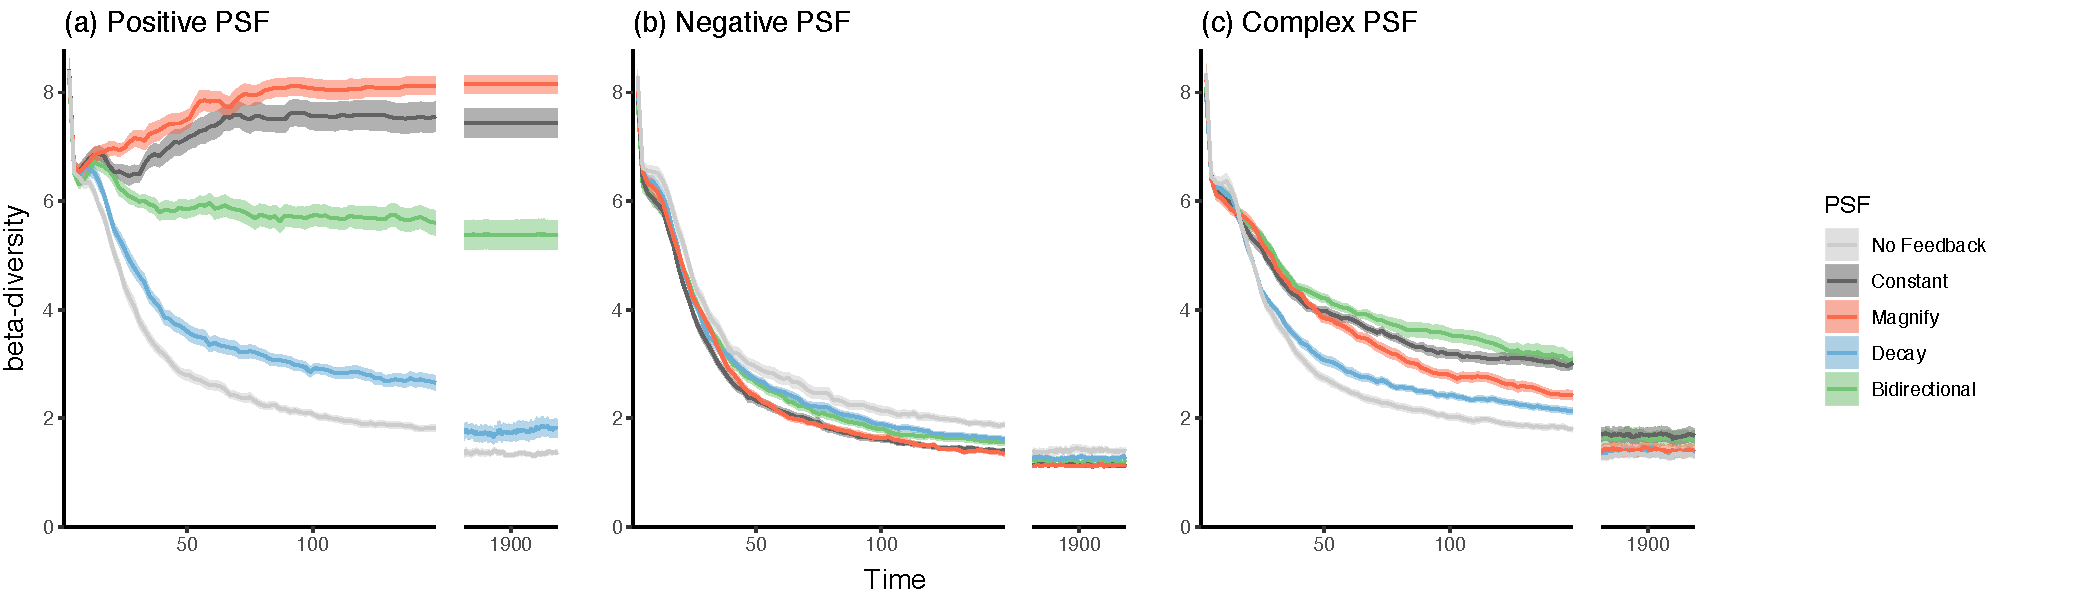
\includegraphics[width=20cm]{Chapter6/Simulation_AllPSF_Aggregate.pdf}}
	\caption[Simulated community convergence patterns under different plant--soil microbe interaction types and different temporal development scenarios.]
		{\hspace{1mm} 
		Simulated community convergence patterns under different plant--soil microbe interaction types and different temporal development scenarios.
		Each panel shows, under different plant--soil microbe interaction types, the temporal trends of beta-diversity (mean $\pm$ SE, $n = 20$) for different temporal development scenarios.
		(a) Positive conspecific plant--soil microbe interactions; (b) Negative conspecific plant--soil microbe interactions; (c) Complex plant--soil microbe interactions.
		Within each plant--soil microbe interaction type, the following temporal development scenarios were considered: 
		No plant--soil microbe interactions (light gray); Constant interaction strengths that are independent to plant age (black); Magnifying interaction strengths that intensify to their biological extremes with increasing plant age (orange); Decaying interaction strengths that attenuate to one with increasing plant age (blue); and Bidirectionally varying interaction strengths that either intensify or attenuate with increasing plant age (green). See Appendix S1 for detailed model description.}
	\label{fig:SimulationAllPSF}
\end{sidewaysfigure}


